% Model report generated by SolverMapp.
% Compile with: pdflatex, bibtex, pdflatex, pdflatex (references.bib is written by the first run).
\begin{filecontents*}[overwrite]{references.bib}
@misc{ref,
  note   = {Discrete marching test},
  key    = {Discrete marching test}
}

@misc{refb,
  note   = {Discrete force balance},
  key    = {Discrete force balance}
}

@misc{clapeyron1834,
  author = {Clapeyron},
  year   = {1834},
  note   = {Thermodynamics 1st law}
}

@misc{refc,
  note   = {Fixed-point convergence},
  key    = {Fixed-point convergence}
}

@misc{van1873,
  author = {van der Waals},
  year   = {1873},
  note   = {Over de continuiteit van den gas- en vloeistoftoestand}
}
\end{filecontents*}
\documentclass[11pt,a4paper]{article}
\usepackage[T1]{fontenc}
\usepackage[utf8]{inputenc}
\usepackage{lmodern}
\usepackage{amsmath,amssymb}
\usepackage{booktabs,longtable}
\usepackage{siunitx}
\usepackage{algorithm}
\usepackage{algpseudocode}
\usepackage{tikz}
\usetikzlibrary{positioning,shapes.geometric,shapes.misc,arrows.meta}
\usepackage{adjustbox}
\usepackage[hidelinks]{hyperref}

\title{Model description}
\author{}
\date{\today}

\begin{document}
\maketitle

The model consists of 5 equations in 14 variables: 9 inputs, 2 state variables, 2 intermediate variables and 1 output. It is solved in 3 steps (Algorithm~\ref{alg:solution}).

\section{Nomenclature}
\begin{longtable}{@{}l p{0.48\linewidth} l l@{}}
  \toprule
  Symbol & Description & Unit & Value \\
  \midrule
  \endhead
  \bottomrule
  \endfoot
  \multicolumn{4}{@{}l}{\textit{Inputs}} \\
  $N$ & Number of force elements & -- & \num{5} \\
  $f_i$ & Element force array & \si{N} & \num{10.0} \\
  $x_1$ & Lower integration bound & \si{m} & \num{0.0} \\
  $x_2$ & Upper integration bound & \si{m} & \num{2.0} \\
  $p$ & Gas pressure & \si{Pa} & \num{5e6} \\
  $a$ & Van der Waals attraction constant (CO2) & \si{Pa.m^{6}/mol^{2}} & \num{0.3640} \\
  $b$ & Van der Waals co-volume (CO2) & \si{m^{3}/mol} & \num{4.267e-5} \\
  $R_u$ & Universal gas constant & \si{J/(mol.K)} & \num{8.314} \\
  $T_g$ & Gas temperature & \si{K} & \num{280} \\
  \addlinespace
  \multicolumn{4}{@{}l}{\textit{State variables}} \\
  $y$ & Marching state variable (y\_0 = 1) & -- & \num{1.0} \\
  $T$ & Converged temperature state & \si{K} & \num{300.0} \\
  \addlinespace
  \multicolumn{4}{@{}l}{\textit{Intermediate variables}} \\
  $F_{total}$ & Accumulated total force & \si{N} &  \\
  $W$ & Integrated work output & \si{J} &  \\
  \addlinespace
  \multicolumn{4}{@{}l}{\textit{Outputs}} \\
  $v$ & Molar volume (start = ideal-gas volume, vapour branch) & \si{m^{3}/mol} &  \\
\end{longtable}

\section{Governing equations}

\subsection{State step recurrence}
Source: \cite{ref}, Eq.~(1).
\begin{equation}
  y_{n+1} = y_n + 1
  \label{eq:state-step-recurrence}
\end{equation}
\noindent where

\noindent\begin{tabular}{@{\quad}l@{\quad}p{0.7\linewidth}@{}}
  $y$ & Marching state variable (y\_0 = 1), dimensionless \\
\end{tabular}

\noindent Marched over 10 steps, starting from the start value of $y$. \textit{Assumptions:} Starts from initial condition y\_0 = 1 and marches N\_steps times.

\subsection{Total force summation}
Source: \cite{refb}, Eq.~(2).
\begin{equation}
  F_{total} = \sum_{i=1}^{N} f_i
  \label{eq:total-force-summation}
\end{equation}
\noindent where

\noindent\begin{tabular}{@{\quad}l@{\quad}p{0.7\linewidth}@{}}
  $F_{total}$ & Accumulated total force, \si{N} \\
  $N$ & Number of force elements, dimensionless \\
  $f_i$ & Element force array, \si{N} \\
\end{tabular}

\noindent Summed over $i = 1, \dots, N$. \textit{Assumptions:} Index i is automatically recognized as a local loop counter.

\subsection{Van der Waals equation of state}
Source: \cite{van1873}, Eq.~(5).
\begin{equation}
  \left(p + \frac{a}{v^2}\right)\left(v - b\right) = R_u T_g
  \label{eq:van-der-waals-equation-of-state}
\end{equation}
\noindent where

\noindent\begin{tabular}{@{\quad}l@{\quad}p{0.7\linewidth}@{}}
  $v$ & Molar volume (start = ideal-gas volume, vapour branch), \si{m^{3}/mol} \\
  $p$ & Gas pressure, \si{Pa} \\
  $a$ & Van der Waals attraction constant (CO2), \si{Pa.m^{6}/mol^{2}} \\
  $b$ & Van der Waals co-volume (CO2), \si{m^{3}/mol} \\
  $R_u$ & Universal gas constant, \si{J/(mol.K)} \\
  $T_g$ & Gas temperature, \si{K} \\
\end{tabular}

\noindent Implicit in $v$: solved for the root of the residual (left side minus right side) by Newton–Raphson iteration from the start value of $v$, until the relative step is below \num{1e-10}, with at most 50 iterations. The iteration is kept on the branch $b \le v$, which selects the root when the equation has several. \textit{Assumptions:} Below the critical temperature the cubic has three roots: liquid, unstable and vapour. The initial guess picks the branch.

\subsection{Boundary work integral}
Source: \cite{clapeyron1834}, Eq.~(3).
\begin{equation}
  W = \int_{x_1}^{x_2} F_{total} \, dx
  \label{eq:boundary-work-integral}
\end{equation}
\noindent where

\noindent\begin{tabular}{@{\quad}l@{\quad}p{0.7\linewidth}@{}}
  $W$ & Integrated work output, \si{J} \\
  $x_1$ & Lower integration bound, \si{m} \\
  $x_2$ & Upper integration bound, \si{m} \\
  $F_{total}$ & Accumulated total force, \si{N} \\
\end{tabular}

\noindent Integrated numerically over $x$ from $x_1$ to $x_2$ with the trapezoidal rule ($n = 100$). \textit{Assumptions:} Evaluated numerically via trapezoidal quadrature.

\subsection{Non-linear relaxation update}
Source: \cite{refc}, Eq.~(4).
\begin{equation}
  T_{new} = 0.5 T_{old} + 0.02 W
  \label{eq:non-linear-relaxation-update}
\end{equation}
\noindent where

\noindent\begin{tabular}{@{\quad}l@{\quad}p{0.7\linewidth}@{}}
  $T$ & Converged temperature state, \si{K} \\
  $W$ & Integrated work output, \si{J} \\
\end{tabular}

\noindent Iterated until the change in $T$ is below \num{1e-6}, with at most 500 iterations. \textit{Assumptions:} Iterates until |T\_new - T\_old| < tol.

\section{Solution algorithm}
\begin{algorithm}[htbp]
  \caption{Solution procedure}\label{alg:solution}
  \begin{algorithmic}[1]
    \State Set the inputs $N$, $f_i$, $x_1$, $x_2$, $p$, $a$, $b$, $R_u$ and $T_g$
    \State Set the start values $y$ = \num{1.0} and $T$ = \num{300.0}
    \For{$n = 1, \dots, 10$}
      \State Update $y$ with Eq.~\eqref{eq:state-step-recurrence}
    \EndFor
    \State Compute $F_{total}$ by the sum in Eq.~\eqref{eq:total-force-summation}
    \State Start from the start value of $v$, branch $b \le v$
    \Repeat \Comment{Newton–Raphson}
      \State $v \leftarrow v - R(v) / R'(v)$, with $R$ the residual of Eq.~\eqref{eq:van-der-waals-equation-of-state}
    \Until{the relative step in $v$ is below \num{1e-10} (at most 50 iterations)}
    \State Compute $W$ by numerical integration of Eq.~\eqref{eq:boundary-work-integral} (trapezoidal rule, $n = 100$)
    \Repeat
      \State Update $T$ with Eq.~\eqref{eq:non-linear-relaxation-update}
    \Until{the change in $T$ is below \num{1e-6} (at most 500 iterations)}
  \end{algorithmic}
\end{algorithm}

Figure~\ref{fig:flowchart} shows the same procedure as a flowchart.

\begin{figure}[htbp]
  \centering
  \begin{adjustbox}{max width=\linewidth, max totalheight=0.9\textheight}
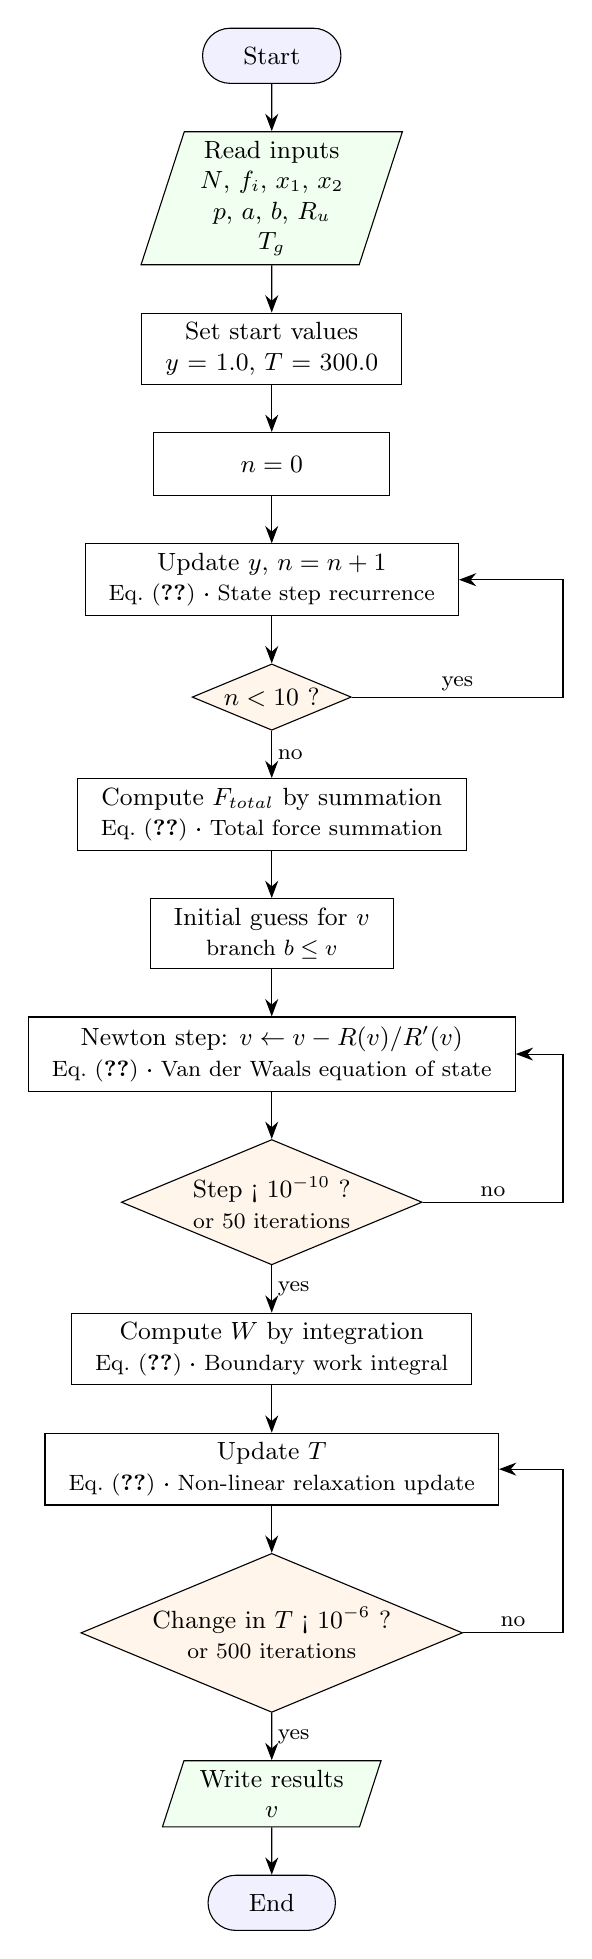
\begin{tikzpicture}[
  node distance=6mm, >={Stealth[length=2.2mm]}, font=\small,
  every node/.style={align=center},
  term/.style={draw, rounded rectangle, minimum height=7mm, inner xsep=5mm, fill=blue!6},
  io/.style={draw, trapezium, trapezium left angle=72, trapezium right angle=108, trapezium stretches body, minimum height=8mm, inner xsep=2mm, fill=green!6},
  proc/.style={draw, rectangle, minimum height=8mm, minimum width=30mm, inner xsep=3mm},
  dec/.style={draw, diamond, aspect=2.4, inner sep=1pt, fill=orange!8},
  lbl/.style={font=\footnotesize, inner sep=2pt}]
  \node[term] (n1) {Start};
  \node[io, below=of n1] (n2) {Read inputs \\ $N$, $f_i$, $x_1$, $x_2$ \\ $p$, $a$, $b$, $R_u$ \\ $T_g$};
  \node[proc, below=of n2] (n3) {Set start values \\ $y$ = 1.0, $T$ = 300.0};
  \node[proc, below=of n3] (n4) {$n = 0$};
  \node[proc, below=of n4] (n5) {Update $y$, $n = n + 1$ \\ {\footnotesize Eq.~\eqref{eq:state-step-recurrence} \textperiodcentered{} State step recurrence}};
  \node[dec, below=of n5] (n6) {$n < 10$ ?};
  \node[proc, below=of n6] (n7) {Compute $F_{total}$ by summation \\ {\footnotesize Eq.~\eqref{eq:total-force-summation} \textperiodcentered{} Total force summation}};
  \node[proc, below=of n7] (n8) {Initial guess for $v$ \\ {\footnotesize branch $b \le v$}};
  \node[proc, below=of n8] (n9) {Newton step: $v \leftarrow v - R(v) / R'(v)$ \\ {\footnotesize Eq.~\eqref{eq:van-der-waals-equation-of-state} \textperiodcentered{} Van der Waals equation of state}};
  \node[dec, below=of n9] (n10) {Step < $10^{-10}$ ? \\ {\footnotesize or 50 iterations}};
  \node[proc, below=of n10] (n11) {Compute $W$ by integration \\ {\footnotesize Eq.~\eqref{eq:boundary-work-integral} \textperiodcentered{} Boundary work integral}};
  \node[proc, below=of n11] (n12) {Update $T$ \\ {\footnotesize Eq.~\eqref{eq:non-linear-relaxation-update} \textperiodcentered{} Non-linear relaxation update}};
  \node[dec, below=of n12] (n13) {Change in $T$ < $10^{-6}$ ? \\ {\footnotesize or 500 iterations}};
  \node[io, below=of n13] (n14) {Write results \\ $v$};
  \node[term, below=of n14] (n15) {End};
  \coordinate (E) at (current bounding box.east);
  \coordinate (L0) at ([xshift=6mm]E);
  \draw[->] (n1) -- (n2);
  \draw[->] (n2) -- (n3);
  \draw[->] (n3) -- (n4);
  \draw[->] (n4) -- (n5);
  \draw[->] (n5) -- (n6);
  \draw[->] (n6) -- node[lbl, right] {no} (n7);
  \draw[->] (n7) -- (n8);
  \draw[->] (n8) -- (n9);
  \draw[->] (n9) -- (n10);
  \draw[->] (n10) -- node[lbl, right] {yes} (n11);
  \draw[->] (n11) -- (n12);
  \draw[->] (n12) -- (n13);
  \draw[->] (n13) -- node[lbl, right] {yes} (n14);
  \draw[->] (n14) -- (n15);
  \draw[->] (n6.east) -- node[lbl, above] {yes} (n6.east -| L0) |- (n5.east);
  \draw[->] (n10.east) -- node[lbl, above] {no} (n10.east -| L0) |- (n9.east);
  \draw[->] (n13.east) -- node[lbl, above] {no} (n13.east -| L0) |- (n12.east);
\end{tikzpicture}
  \end{adjustbox}
  \caption{Flowchart of the solution procedure}\label{fig:flowchart}
\end{figure}

\bibliographystyle{plain}
\bibliography{references}

\end{document}